\documentclass[10pt,a4paper]{article}
\usepackage{fullpage}
\usepackage{graphicx}

\usepackage{fancyhdr}
\setlength{\headheight}{13pt}
\pagestyle{fancy}

% default sans-serif
\renewcommand{\familydefault}{\sfdefault}

% no lines for headers and footers
\renewcommand{\headrulewidth}{0pt}
\renewcommand{\footrulewidth}{0pt}

% header
\fancyhf{}
\lhead{GWD-R}
\rhead{\today}

% footer
\lfoot{occi-wg@ogf.org}
\rfoot{\thepage}

% paragraphs need some space...
\setlength{\parindent}{0pt}
\setlength{\parskip}{1ex plus 0.5ex minus 0.2ex}

% some space between header and text...
\headsep 13pt

\setcounter{secnumdepth}{4}

\begin{document}

% header on first page is different
\thispagestyle{empty}

GWD-R \hfill  Thijs Metsch, Platform Computing\\
OCCI-WG \hfill  Andy Edmonds, Intel\\
\rightline {October 7, 2010}\\
\rightline {Updated: \today}

\vspace*{0.5in}

\begin{Large}
\textbf{Open Cloud Computing Interface - HTTP Rendering}
\end{Large}

\vspace*{0.5in}

\underline{Status of this Document}

This document provides information to the community regarding the specification of the Open Cloud Computing Interface. Distribution is unlimited.

\underline{Obsoletes}

This document obsoletes GFD-xxx [REFERENCE].

\underline{Copyright Notice}

Copyright \copyright Open Grid Forum (2009-2010). All Rights Reserved.

\underline{Trademarks}

OCCI is a trademark of the Open Grid Forum.

\underline{Abstract}

This document, part of a document series, produced by the OCCI working group within the Open Grid Forum (OGF), provides a high-level definition of a Protocol and API. The document is based upon previously gathered requirements and focuses on the scope of important capabilities required to support modern service offerings. 

\tableofcontents

\section{Introduction}

The Open Cloud Computing Interface (OCCI) is a RESTful Protocol (and API) for all kinds of Management tasks. Originally initiated to create a remote management API for IaaS model based Services, allowing for the development of interoperable tools for common tasks including deployment, autonomic scaling and monitoring, it now can be used to severe other models as well. To be modular and extensible the current specification itself is currently split into three complimentary documents:

\begin{itemize}
\item Core – this defines the OCCI model
\item HTTP Rendering - this defines how to manipulate the core model using the OCCI RESTful API. The document defines how the OCCI model can be communicated and thus serialized using HTTP.
\item Infrastructure – this defines the infrastructure domain resource types, the required attributes for each and the actions that can be taken on each.
\end{itemize}

\section{Notational Conventions}

All these parts and the information within are mandatory for implementors (unless otherwise specified). The key words "MUST", "MUST NOT", "REQUIRED", "SHALL", "SHALL NOT", "SHOULD", "SHOULD NOT", "RECOMMENDED", "MAY", and "OPTIONAL" in this document are to be interpreted as described in RFC 2119. 

UML activity diagrams do not specify how OCCI should be rendered but what possible request and outcomes can be.

\section{HTTP Rendering}

\textbf{TBD: Explain CRUD/REST here....}

\subsection{Versioning}

Required: User-agent - server...

\subsection{Content-type and Accept headers}

Required: Accept - Content-type

\textbf{TBD: describe stuff here.... Impl should react on Accept and Content-type stuff...}

\subsection{Behaviour of HTTP operations}

\paragraph{The HTTP POST Operation behaviour}

The UML diagram \ref{fig:post_operation} shows what the Server can return, and what it will return when performing an POST operation.

\begin{figure}[h!]
	\centering
	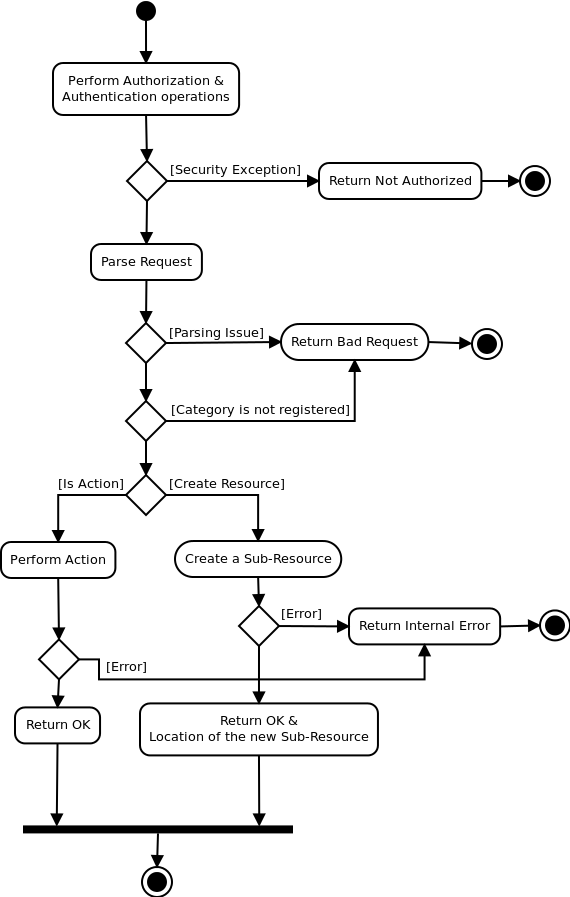
\includegraphics[scale=0.4]{dia/POST_operation.png}
	\caption{Behaviour for HTTP Post}
	\label{fig:post_operation}
\end{figure}

The OCCI service implemetation MUST create sub resource of and existing URN (which can be Root). Action must be exposed by adding \emph{;action=<action term>} to the URI.

\subsection{Render OCCI model in the HTTP Header}

\textbf{Note:} This is the default rendering mode for OCCI - It is the fallback. In some use cases (Collections, Query Interface) it needs to render stuff using specific Content-types like \textit{'text/uri-list'} or \textit{'text/plain'}

The HTTP header fields MUST follow the specification in RFC 2616. A header field consists of a name followed by a colon (":") and the field value. The format of the field value is specified separately for each of the three header fields, see below.

HTTP header fields MAY appear multiple times in a HTTP request or response. In order to be OCCI compliant the specification of multiple message-header fields according to RFC 2616 (section 4.2) MUST be fully supported. In essence there are two valid representation of multiple HTTP header field values. A header field might either appear several times or as a single header field with a comma-separated list of field values. Due to implementation issues in many web frameworks and client libraries it is RECOMMENDED to use the comma-separated list format for best interoperability.

HTTP header field values which contain separator characters MUST be properly quoted according to RFC 2616.

\subsubsection{HTTP Header Fields}

Three different HTTP header fields are used to render the OCCI model. Each header field value has a different format.

\paragraph{Category Header}

The Category header is defined by the Web Categories specification, http://tools.ietf.org/html/draft-johnston-http-category-header-01. The semantics of the Category header in the OCCI context is described in the OCCI Core \& Models document.

\begin{verbatim}
Category:<term>;scheme="<scheme>"
    [;rel=<Comma seperated list of <scheme> + '#' + <term> of related categories>]
    [;attributes=<comma seperated list of attribute names>]
    [;title=<Title of this Category>]    
\end{verbatim}

There is no order for the optional part.

\paragraph{Link Header}

The Link header is defined by the Web Linking specification, http://tools.ietf.org/html/draft-nottingham-http-link-header-10. The semantics of the Link header in the OCCI context is described in the OCCI Core \& Models document.

\begin{verbatim}
Link:???

or in case it is an Action:

Link:<<URL of the resource>> + ";action=" + <Term of the action>
\end{verbatim}

\paragraph{X-OCCI-Attribute Header}

The Attribute header is used to render the attributes associated with a OCCI Resource. A simple key-value format is used. The field value consist of an attribute name followed by an equal sign ("=") and the attribute value. The attribute value must be quoted if it includes a separator character, see RFC 2616 (page 16).

\paragraph{X-OCCI-Location Header}

\ldots

\begin{verbatim}
Attribute:<list of comma separated <attribute name>=<attribute value> pairs>
\end{verbatim}

Valid attribute names for OCCI Resources are specified in appropiate Extension documents.

\subsubsection{Rendering the OCCI model}

The following setups show how the Core Model MUST be rendered. Shown are the HTTP Header fiels which MUST be available in a request from the Client or a response from the Server.

\paragraph{Rendering of a Category}
\begin{verbatim}
Required: Category
Optional: N/A
\end{verbatim}

\paragraph{Rendering of a Kind}
\begin{verbatim}
Required: Category
Optional: N/A
\end{verbatim}

\paragraph{Rendering of a Resource}
\begin{verbatim}
Required: Category
Optional: Attribute, Link
\end{verbatim}

\paragraph{Rendering of a Action}
\begin{verbatim}
Required: Category, Link
Optional: Attribute
\end{verbatim}

\paragraph{Rendering of a Link}
\begin{verbatim}
Required: Category, Link
Optional: Attribute
\end{verbatim}
Please note that Link and Action are rendered almost equaly.

\subsection{Render OCCI model in the HTTP Body}
%
%When using this rendering the Server must indicate that it Accept's and uses the 'text/plain' Content-Type and Accept Header fields.
%Note: In case that the Header Attributes become overfull, or collections are used the OCCI model MUST be rendered in the HTTP-Body. This MUST also be done when the Client requests 'text/plain'.
%
%See above just that Category, Link and Attribute are now in the body... And ':' becomes '='
%
\subsection{Render OCCI model via URL Listings}

%Note: This rendering cannot render Kinds of Categories directly but just Links to them. For concrete rendering of Kinds and Categories the Content-types '*/*', 'text/plain' must be used.

\section{Contributors}

Editors: Andy Edmonds, Thijs Metsch \\
Contributors: Alexander Papaspyrou, Ralf Nyrén, Sam Johnston

\textbf{TBD: Bunch op people missing here - create table\ldots}

\section{Appendix}

\subsection{Examples for rendering the OCCI model in the HTTP Header}

\subsubsection{Triggering an Action}

\begin{verbatim}
\end{verbatim}

\subsubsection{Listing Resource}

\begin{verbatim}
> GET / HTTP/1.1
> User-Agent: curl/7.21.0 (x86_64-pc-linux-gnu) libcurl/7.21.0 OpenSSL/0.9.8o zlib/1.2.3.4 libidn/1.18
> Host: localhost:8080
> Accept: */*

< HTTP/1.1 200 OK
< Location: /4147377d-283d-4947-8696-7c1591e89179
< Transfer-Encoding: chunked
< Date: Mon, 11 Oct 2010 15:11:05 GMT
< Server: CherryPy/3.1.2 WSGI Server
<
< 0
<
\end{verbatim}

\subsubsection{Request with missing Category rendering}

\begin{verbatim}
> PUT /21d0171e-6de3-40ab-b595-25e5de607ccc HTTP/1.1
> User-Agent: curl/7.21.0 (x86_64-pc-linux-gnu) libcurl/7.21.0 OpenSSL/0.9.8o zlib/1.2.3.4 libidn/1.18
> Host: localhost:8080
> Accept: */*

< HTTP/1.1 400 Bad Request
< Content-Type: text/html
< Transfer-Encoding: chunked
< Date: Mon, 11 Oct 2010 15:07:21 GMT
< Server: CherryPy/3.1.2 WSGI Server
< 
< (BadRequest('400 Bad Request',), 'No categories could be found in the header!')
\end{verbatim}

\subsection{Examples for rendering the OCCI model with uri-lists}

\subsection{Examples for rendering the OCCI model in the HTTP Body}

\section{Glossary}

\begin{tabular}{l|l}
Term & Description \\
\hline
OCCI & Open Cloud Computing Interface \\
URN & Unified Resource Name \\
URL & TBD \\
URI & TBD \\
\end{tabular}

\section{Intellectual Property Statement}

The OGF takes no position regarding the validity or scope of any intellectual property or other rights that might be claimed to pertain to the implementation or use of the technology described in this document or the extent to which any license under such rights might or might not be available; neither does it represent that it has made any effort to identify any such rights. Copies of claims of rights made available for publication and any assurances of licenses to be made available, or the result of an attempt made to obtain a general license or permission for the use of such proprietary rights by implementers or users of this specification can be obtained from the OGF Secretariat.

The OGF invites any interested party to bring to its attention any copyrights, patents or patent applications, or other proprietary rights which may cover technology that may be required to practice this recommendation. Please address the information to the OGF Executive Director.

\section{Disclaimer}

This document and the information contained herein is provided on an ''As Is'' basis and the OGF disclaims all warranties, express or implied, including but not limited to any warranty that the use of the information herein will not infringe any rights or any implied warranties of merchantability or fitness for a particular purpose.

\section{Full Copyright Notice}

Copyright \copyright Open Grid Forum (2009-2010). All Rights Reserved.

This document and translations of it may be copied and furnished to others, and derivative works that comment on or otherwise explain it or assist in its implementation may be prepared, copied, published and distributed, in whole or in part, without restriction of any kind, provided that the above copyright notice and this paragraph are included on all such copies and derivative works. However, this document itself may not be modified in any way, such as by removing the copyright notice or references to the OGF or other organizations, except as needed for the purpose of developing Grid Recommendations in which case the procedures for copyrights defined in the OGF Document process must be followed, or as required to translate it into languages other than English.

The limited permissions granted above are perpetual and will not be revoked by the OGF or its successors or assignees.

\section{References}

Note that only permanent documents should be cited as references. Other items, such as Web pages or working groups, should be cited inline (i.e., see the Open Grid Forum, http://www.ogf.org). References should conform to a standard such as used by IEEE/ACM, MLA, Chicago or similar. Include an author, year, title, publisher, place of publication. For online materials, also add a URL. It is acceptable to separate out ''normative references,'' as IETF documents typically do. Some sample citations: 

\end{document}
